%%%%%%%%%%%%%%%%%%%%%%%%%%%%%%%%%%%%%%%%%%%%%%%%%%%%%%%%%%%%%%%%%%%%%%%%%%%%%
%	e-Yantra, IIT-Bombay

%	Document Author: Abhishek Rathore, G. Harshawardhan
%	Date: 04-July,2016 

%%%%%%%%%%%%%%%%%%%%%%%%%%%%%%%%%%%%%%%%%%%%%%%%%%%%%%%%%%%%%%%%%%%%%%%%%%%%%

\documentclass[11pt,a4paper]{article}

\usepackage{graphicx}
\usepackage{listings}
\usepackage{url}
\usepackage{float}
\usepackage{subcaption}
\title{Tutorial on Object  Tracking using a Pi-Cam interfaced on a Raspberry-Pi}
\author{e-Yantra Team}
\date{\today}

\begin{document}
	\maketitle
	\newpage
	\tableofcontents
	\newpage
	\section{Object  Tracking using a Pi-Cam interfaced on a Raspberry-Pi}
	\textbf{Objective} of this tutorial is to track a object from a given Region-Of-Interest and move the camera according to the object movement using servos.
	\section{Prerequisites}
	\begin{itemize}
		\item Pan-Tilt Camera system interafced R-Pi
		\item Python and Open CV installed on the R-Pi
	\end{itemize}
	\section{Hardware Requirement}
	\begin{itemize}
		\item Raspberry-Pi B+ Development Board
		\item Raspberry-Pi Camera Module(Pi Camera)
		\item Ethernet Cable/Wifi Mdoule
		\item Camera mount frame
	\end{itemize}
	\section{Software Requirement}
	\begin{itemize}
		\item Python 2.7.11
		\item OpenCV 2.4.13 
		\item numpy 1.7.1
		\item RPIO and picamera packages
        \item \textbf{Note :} These are the versions we were working on while creating this tutorial.
	\end{itemize}
	\section{Theory and Description}
	Here We will be moving the camera according to the object movement in the frame so that the camera always tries to keep the object at its center.
	\par To make the camera servos move in both Pitch and Roll directions at the same time simultaneously which is not possible as the servos don't have a feedback of how much distance they had moved or the angle they are in present state,and also we cant get a feedback through the center as both the camera and servos need the center at the same time for tracking and movement respectively.
	\par This center controversy can be solved by multi-processing,in which we assign each Roll and Pitch servo a process in which they will be two global variables (one is Current Position of the servo and the second is Desired Position of the servo).These processes will be executing in the back-end all the time,but gets updated only when they get called by a function which updates the two global variables.   
	\par For the distance to be moved by the servos as we don't have a feedback from the servo,we can use the proportionality constant which can be obtained by calibrating the servos several times.
	\newline
	\textbf{Note:}We can also use PID controller for which we need to know the Integration and Derivation constants. 
	 \vspace{1cm}
	 \par\textbf{CAMShift} tracking is done parallel to this camera movement in which again a center controversy may arise.Here as we know that the CAM shift works on the previous track window and previous center which will be a totally different co-ordinates when the camera moves frequently.
	 \par We can solve this as we know that camera always tries to keep the object at its center.So we gave the CAM shift its previous track window as the camera center.
	 \par \textbf{Here issues may arise about "Is the servo fast enough to catch-up with the CAM shift track by keeping the object at its center every time?"}
	 \par  As we know the servos work in a totally different processes ,they are fast enough to meet up our needs of the CAM Shift track window (which we took a 20x20 square from the center).The implementation of this is shown in the below sections.
	
	\section{Experiment}
	The Python code is given below
	\lstinputlisting[language=Python]{code.py}
  	\section{References}
	The idea of using multi-processing is taken from ServoBlaster package used in R-Pi for  multiple servo controlling written by Richard Hirst.
	
	\begin{enumerate}
	\item \url{https://github.com/richardghirst/PiBits/tree/master/ServoBlaster}

     \item \url{https://www.raspberrypi.org/forums/viewtopic.php?f=44&t=54067}
     \item \url{https://www.youtube.com/watch?v=m99n2heDXE87}
      \item \url{http://www.instructables.com/id/Raspberry-Pi-Ball-tracking/}
   \end{enumerate}
 \newpage
	\section{Exercise}
	Object tracking with camera movement is shown below.
	\begin{figure}[h]
     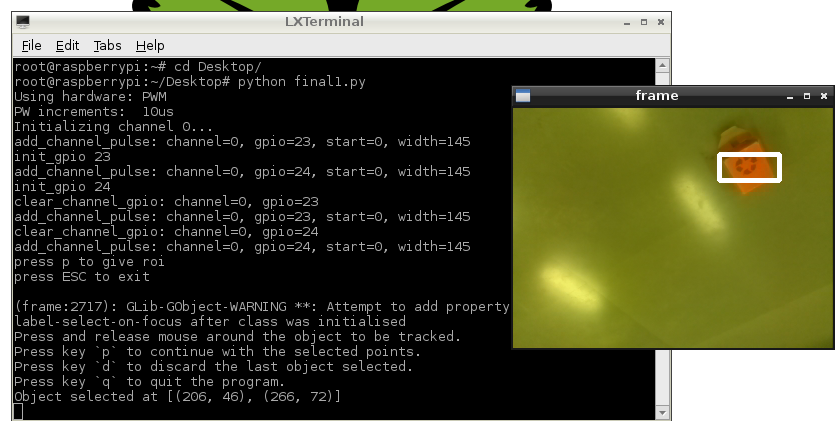
\includegraphics[scale=0.5]{1.png}
   \centering
 \caption{Selction of object through ROI}
  \end{figure}
  \begin{figure}[h]
 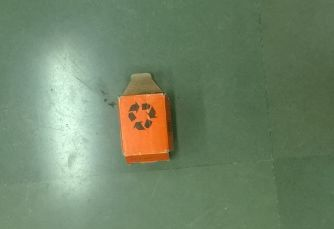
\includegraphics[scale=0.5]{s1.jpg}
   \centering
 \caption{Initial position of the object}
  \end{figure}
  \begin{figure}[h]
 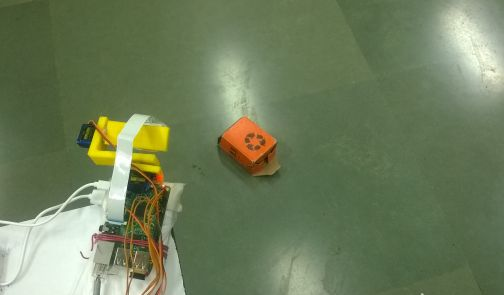
\includegraphics[scale=0.5]{s2.jpg}
   \centering
 \caption{Object slightly moved to left}
  \end{figure}
   \begin{figure}[h]
    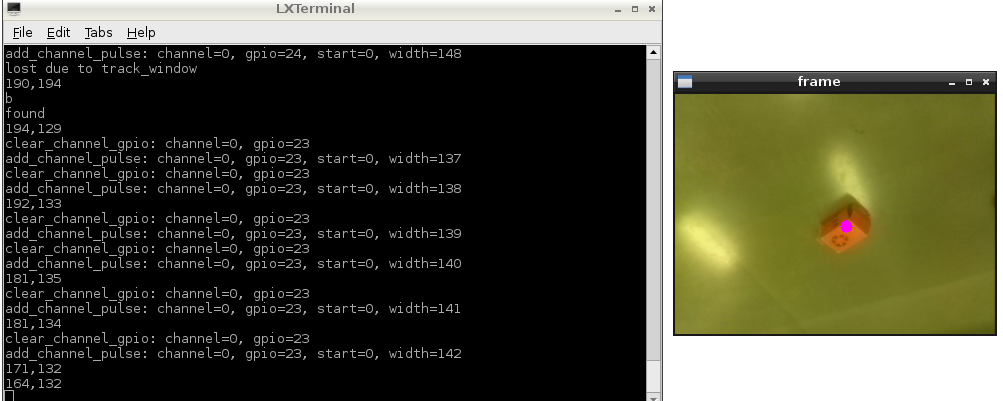
\includegraphics[scale=0.5]{2.png}
   \centering
 \caption{Camera also slightly moved to left}
  \end{figure}
   \begin{figure}[h]
 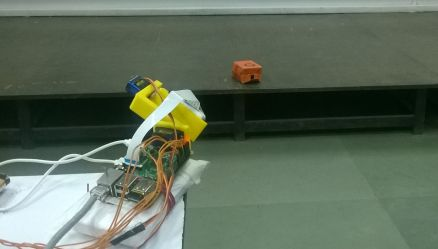
\includegraphics[scale=0.5]{s3.jpg}
   \centering
 \caption{Object largely deviated}
  \end{figure}
   \begin{figure}[h]
    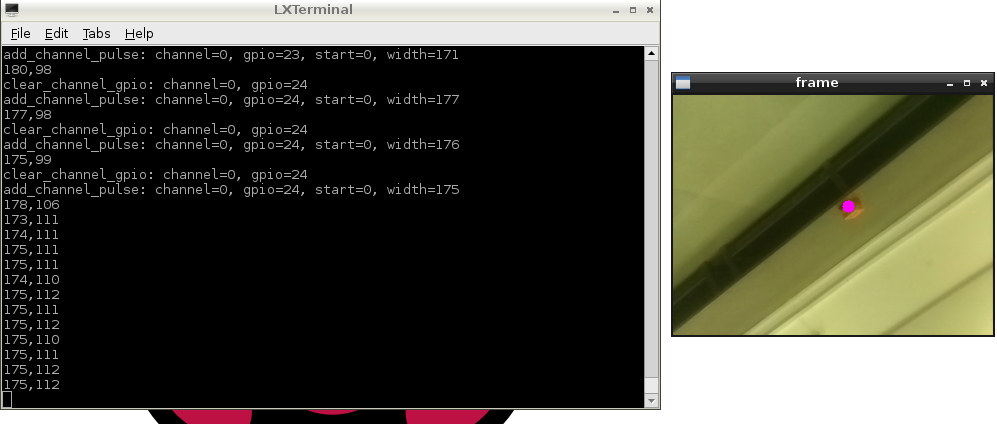
\includegraphics[scale=0.5]{3.png}
   \centering
 \caption{Camera sucessfully catching up with the object}
  \end{figure}
	
	
\end{document}



